
%%%%%%%%%%%%%%%%%%%%%%%%%%%%%%%%%%%%%%%%%
% Beamer Presentation
% LaTeX Template
% Version 1.0 (10/11/12)
%
% This template has been downloaded from:
    % http://www.LaTeXTemplates.com
%
% License:
    % CC BY-NC-SA 3.0 (http://creativecommons.org/licenses/by-nc-sa/3.0/)
%
%%%%%%%%%%%%%%%%%%%%%%%%%%%%%%%%%%%%%%%%%

%----------------------------------------------------------------------------------------
    %   PACKAGES AND THEMES
%----------------------------------------------------------------------------------------
    
    \documentclass{beamer}

\mode<presentation> {
    
    % The Beamer class comes with a number of default slide themes
    % which change the colors and layouts of slides. Below this is a list
    % of all the themes, uncomment each in turn to see what they look like.
    
    %\usetheme{default}
    %\usetheme{AnnArbor}
    %\usetheme{Antibes}
    %\usetheme{Bergen}
    %\usetheme{Berkeley}
    %\usetheme{Berlin}
    %\usetheme{Boadilla}
    %\usetheme{CambridgeUS}
    %\usetheme{Copenhagen}
    %\usetheme{Darmstadt}
    %\usetheme{Dresden}
    %\usetheme{Frankfurt}
    %\usetheme{Goettingen}
    %\usetheme{Hannover}
    %\usetheme{Ilmenau}
    %\usetheme{JuanLesPins}
    %\usetheme{Luebeck}
    \usetheme{Madrid}
    %\usetheme{Malmoe}
    %\usetheme{Marburg}
    %\usetheme{Montpellier}
    %\usetheme{PaloAlto}
    %\usetheme{Pittsburgh}
    %\usetheme{Rochester}
    %\usetheme{Singapore}
    %\usetheme{Szeged}
    %\usetheme{Warsaw}
    
    % As well as themes, the Beamer class has a number of color themes
    % for any slide theme. Uncomment each of these in turn to see how it
    % changes the colors of your current slide theme.
    
    %\usecolortheme{albatross}
    %\usecolortheme{beaver}
    %\usecolortheme{beetle}
    %\usecolortheme{crane}
    %\usecolortheme{dolphin}
    %\usecolortheme{dove}
    %\usecolortheme{fly}
    %\usecolortheme{lily}
    %\usecolortheme{orchid}
    %\usecolortheme{rose}
    %\usecolortheme{seagull}
    %\usecolortheme{seahorse}
    %\usecolortheme{whale}
    %\usecolortheme{wolverine}
    
    %\setbeamertemplate{footline} % To remove the footer line in all slides uncomment this line
    %\setbeamertemplate{footline}[page number] % To replace the footer line in all slides with a simple slide count uncomment this line
    
    %\setbeamertemplate{navigation symbols}{} % To remove the navigation symbols from the bottom of all slides uncomment this line
}

\usepackage{graphicx} % Allows including images
\usepackage{tabularx}
\usepackage{booktabs} % Allows the use of \toprule, \midrule and \bottomrule in tables

\newcommand{\etal}{\emph{et al.}}

%----------------------------------------------------------------------------------------
    %   TITLE PAGE
%----------------------------------------------------------------------------------------
    
    \title[Estimating the Red Queen]{Quantifying the effects of parasites on the maintenance of sex} % The short title appears at the bottom of every slide, the full title is only on the title page

\author{Sang Woo Park} % Your name
\date{\today} % Date, can be changed to a custom date

\begin{document}

\begin{frame}
\titlepage % Print the title page as the first slide
\end{frame}

\begin{frame}{Evolution of sex}
\begin{itemize}
    \item \textbf{Two-fold cost of sex}: (1) cost of producing males and (2) cost of meiosis
    \item the two-fold cost of cost of sex asumes that \textbf{all else is equal}
    \item only 0.01\% eukaryotes conform to purely asexual reproduction. How?
\end{itemize}
\end{frame}

\begin{frame}{Red Queen Hypothesis}
\begin{minipage}[c]{0.55\textwidth}
\begin{itemize}
    \item sexual reproduction creates rare genotypes that can escape infection (\textbf{negative frequncy dependence})
    \item snail population in New Zealand (host for sterilizing trematode infection) is believed to support the hypothesis \cite{vergara2014infection}
    \item prevalence of sex should be \textbf{positively correlated} with prevalence of infection \cite{lively2001trematode}
    \item unable to detect any correlation in a similar snail-trematode system. Why? \cite{dagan2013clonal}
\end{itemize}
\end{minipage}
\begin{minipage}[c]{0.4\textwidth}
\begin{figure}
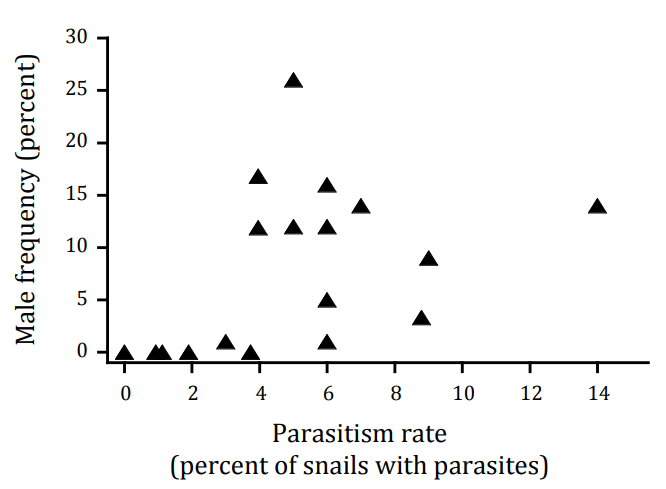
\includegraphics[width=0.9\textwidth]{McKone.png}
\caption{Prevalence of infection is positively correlated with male frequency \cite{mckone2016fine}.}
\vspace{-1em}
\end{figure}
\end{minipage}
\end{frame}

\begin{frame}{Mathematical model}
\begin{figure}
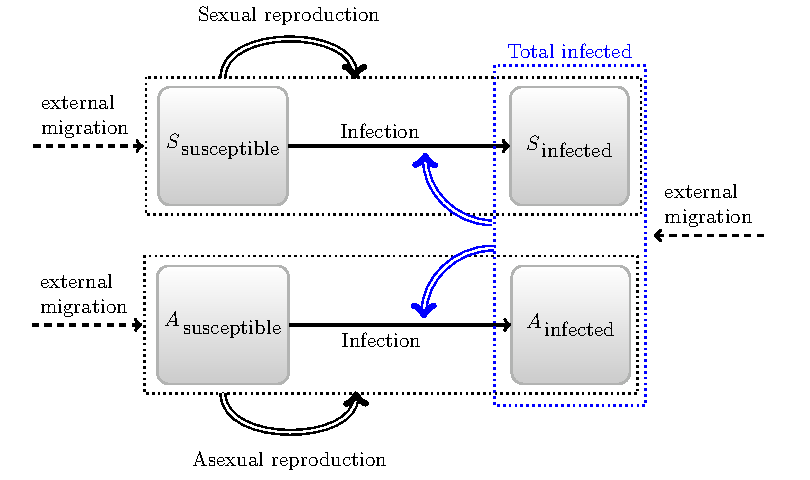
\includegraphics[width=0.5\textwidth]{../fig/model_diagram.pdf}
\caption{Graphical representation of the model. Double lined arrows represent dynamics that are affected by mixing betwee habitats.}
\vspace{-1em}
\end{figure}
\begin{itemize}
    \item competition of obligate sexual v.s. obligate asexual hosts under parasite selection. Hosts are assumed to be diploids and parasites are assumed to be haploids \cite{lively2010epidemiological}
\end{itemize}
\end{frame}

\begin{frame}
\begin{itemize}
    \item offsrpings produced by hosts from a site:
    $$
    \begin{cases}
    S_{ij}' = c_b (1-s) \left(W_U S_{ij,U} (t) + W_I S_{ij,I} (t)\right)\\
    A_{ij}' = W_U A_{ij,U} (t) + W_I A_{ij,I} (t)
    \end{cases}
    $$
    $S_{ij}'$ then goes through recombination and segregation after. Virulence is defined as $V = 1-W_I/W_U$.
    \item expected offsprings in site $k$ in next generation accounting for mixing between sites:
    $$
    \mathrm{E}\left(X_{ij}^k(t+1)\right) = (1 - \epsilon_{\textrm{site}}) X_{ij}^k + \frac{\epsilon_{\textrm{site}}}{n_{\textrm{site}}-1} \sum_{l \neq k} X_{ij}^l,
    $$
    where $X$ can be replaced with either $A$ or $S$.
    \item number of offsprings is taken as a poisson random variable 
\end{itemize}
\vfill
$s$: frequency of males, $W_U$ and $W_I$: fitness of uninfected and infected hosts, $c_b$ scaling factor for cost of sex, $\epsilon_{\textrm{site}}$: mixing between sites
\end{frame}

\begin{frame}
\begin{itemize}
    \item poisson mean number of exposures caused by parasites $i$:
    $$
    \lambda_i^k = \frac{\beta^k}{2 N^k(t+1)} I_i',
    $$
    where $I_i'$ is the number of hosts infected by parasite $i$ after accounting for recombination.
    \item accounting for mixing between sites:
    $$
    \lambda_{i, \textrm{total}}^k = (1 - \epsilon_{\textrm{site}}) \lambda_i^k  + \frac{\epsilon_{\textrm{site}}}{n_{\textrm{site}}-1} \sum_{l \neq k} \lambda_i^l
    $$
    \item force of infection: $\mathrm{FOI}_{ij}^k = \lambda_{i, \textrm{total}}^k + \lambda_{j, \textrm{total}}^k$.
    \item infection is modeled using a binomial random variable with
    $P_{ij}^k(t+1) = 1 - \exp\left(\mathrm{FOI}_{ij}^k\right)$.
\end{itemize}
\vfill
$\beta^k$: the transmission rate at each site.
\end{frame}

\begin{frame}{Simulation}
\begin{itemize}
    \item transmission rate is randomly drawn from a lognormal distribution with parameters $\beta_{\textrm{meanlog}}, \beta_{\textrm{sdlog}}$
    \item number of asexual genotypes present in the system is fixed to $G_{\textrm{asex}}$
    \item sexual hosts are allowed to mix under parasite selection without asexual hosts for 500 generations; then, asexual hosts are introduced and the simulation runs for 600 generations
\end{itemize}
\vfill
\end{frame}

\begin{frame}{Approximate Bayesian Computation}
\begin{itemize}
    \item fitted to two spatial data \cite{dagan2013clonal, mckone2016fine} and one spatio temporal data \cite{vergara2014infection}
    \item prior distribution on $\beta_{\textrm{meanlog}}, \beta_{\textrm{sdlog}}, c_b, \epsilon_{\textrm{site}}, V, G_{\textrm{asex}}$. Rest are fixed.
    \item almost uninformative priors for all except $c_b$; it was scaled to approximately match the 95\% CI for cost of sex reported by \cite{gibson2017two}
    \item considered absolute difference in summary statistics: mean prevalence of sex and infection and CV in mean prevalence of sex and infection across generations/sites
\end{itemize}
\vfill
\resizebox{\textwidth}{!}{
\begin{tabular}{cccc}
\toprule
Parameters &  Dagan \etal\ \cite{dagan2013clonal} & McKone \etal\ \cite{mckone2016fine} & Vergara \etal\ \cite{vergara2014infection} \\
\midrule
$\beta_{\textrm{meanlog}}$   & \multicolumn{2}{c}{$\mathrm{Cauchy}(\textrm{location}=0, \textrm{scale}=2)$} & $\mathrm{Cauchy}(\textrm{location}=2, \textrm{scale}=1)$\\
$\beta_{\textrm{sdlog}}$ & \multicolumn{3}{c}{$\mathrm{Lognormal}(\textrm{meanlog}=0, \textrm{sdlog}=2)$}  \\
$c_b$ & \multicolumn{3}{c}{$\mathrm{Lognormal}(\textrm{meanlog}=-0.1, \textrm{sdlog}=0.1)$} \\
$\epsilon_{\textrm{site}}$  &  $\mathrm{Beta}(\textrm{shape1}=1, \textrm{shape2}=9)$  & $\mathrm{Beta}(\textrm{shape1}=2, \textrm{shape2}=8)$  & $\mathrm{Beta}(\textrm{shape1}=1, \textrm{shape2}=9)$ \\
$V$ & \multicolumn{3}{c}{$\mathrm{Beta}(\textrm{shape1}=6, \textrm{shape2}=2)$} \\
$G_{\textrm{asex}}$ & $\mathrm{BetaBinom}(\textrm{size}=9, \textrm{prob}=5/9, \textrm{theta}=5)+1$ & \multicolumn{2}{c}{$\mathrm{BetaBinom}(\textrm{size}=9, \textrm{prob}=3/9, \textrm{theta}=5)+1$} \\
\bottomrule
\end{tabular}
}
\end{frame}

\begin{frame}{Sequential Monte Carlo}
\begin{itemize}
    \item way to approximate the posterior more efficiently
    \item perform ABC with high tolerance; perform ABC again but draw a weighted sample from the accepted values instead and "jump"
    \item modified Population Monte Carlo suggested by \cite{turner2012tutorial}. Parameters were transformed to an unconstrained scale (possible for all except $G_{\textrm{asex}}$) and jump through gaussian kernel independently for each parameter:
    $$
    q(\cdot | \theta_i^\ast) \sim \mathrm{Normal}(\mu = \theta_i^\ast, \sigma^2 = 2\mathrm{Var}(\theta_{i, t-1})),
    $$
    where $\theta_i^\ast$ is the $i$-th parameter of a transformed accepted parameter sample, $\theta^\ast$, from the last run (a sample we're jumping from) and $\theta_{t-1}$ is the marginal set of accepted $i$-th parameters from the last run,
    \item binomial jump for $G_{\textrm{asex}}$ but prevent it from fixing:
    $$
    q(\cdot | G_{\textrm{asex}}^\ast) \sim \mathrm{Binomial}(\textrm{size}=9, p=(G_{\textrm{asex}}^\ast-0.5)/10)) + 1
    $$
\end{itemize}
\end{frame}

\begin{frame}{Result - ABC}
\begin{figure}
\vspace{-1em}
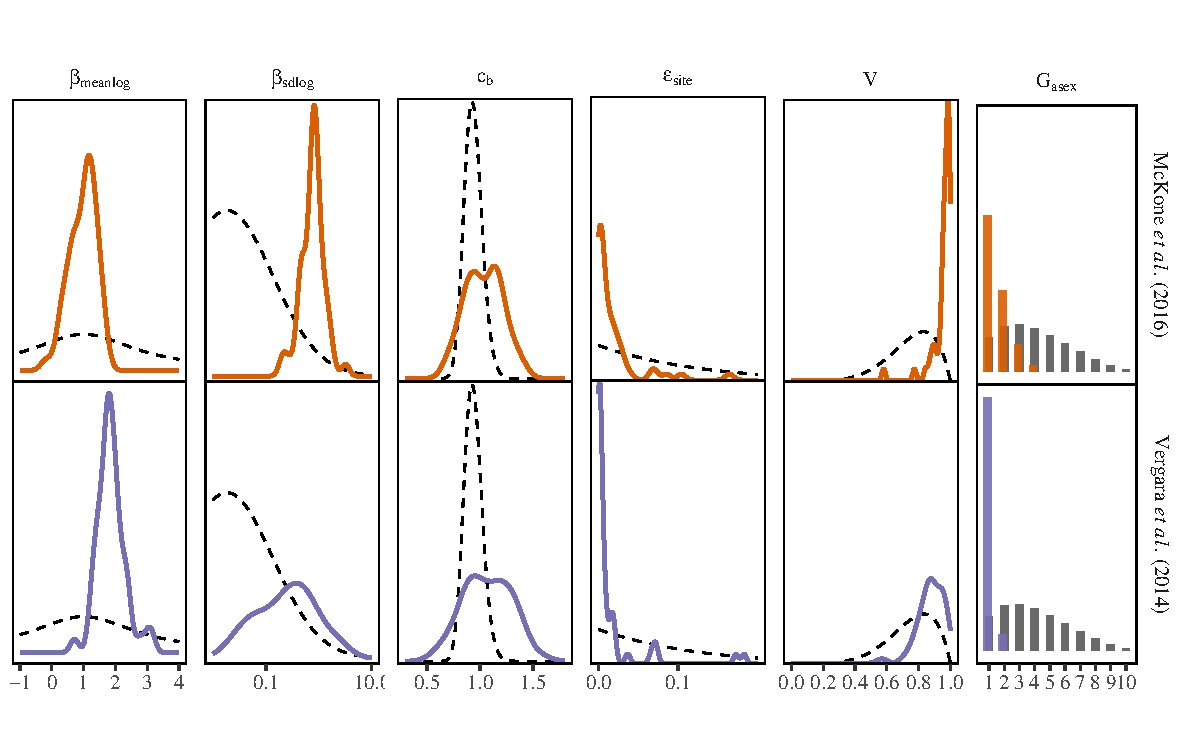
\includegraphics[width=0.9\textwidth]{../fig/smc_param.pdf}
\caption{(black) prior distributions where parameters sampled from and (red) posterior distributions obtained from ABC}
\vspace{-1em}
\end{figure}
\end{frame}

\begin{frame}{Result - simulated data v.s. observed data}
\vspace{-1em}
\begin{figure}
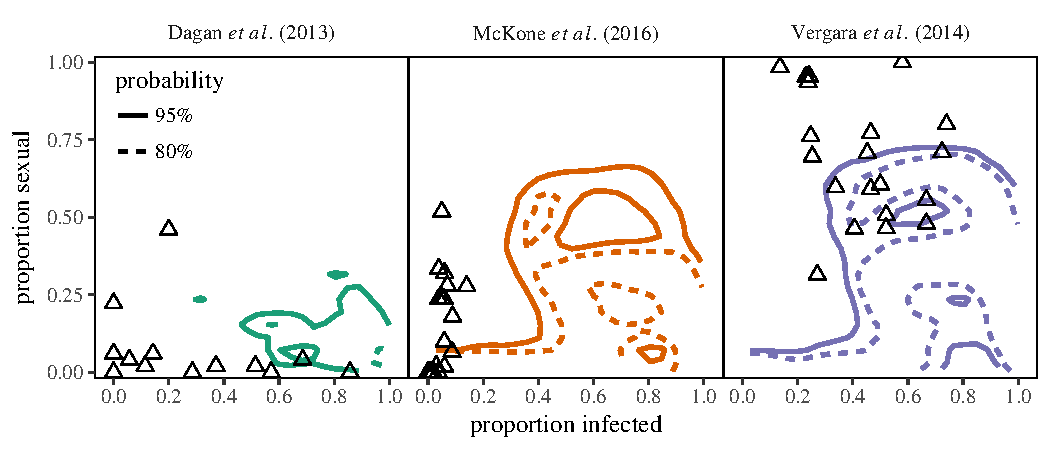
\includegraphics[width=0.8\textwidth]{../fig/simulated_data.pdf}
\vspace{-1em}
\caption{Simulated data v.s. observed data. Each point for simulated data represents mean proportion infected and sexual at each site.}
\vspace{-1em}
\end{figure}
\begin{itemize}
    \item overestimates proportion infected when fitted to McKone \etal\ \cite{mckone2016fine}
    \item spatial structure allows high level of infection to be maintained even at high virulence (middle panel)
    \item initially increasing prevalence of sexual reproduction pulls back infection (consistent with \cite{lively2001trematode}) and causes prevalence of infection to decrease; quadratic overall?
\end{itemize}
\end{frame}

\begin{frame}{Result - Power analysis}
\begin{figure}
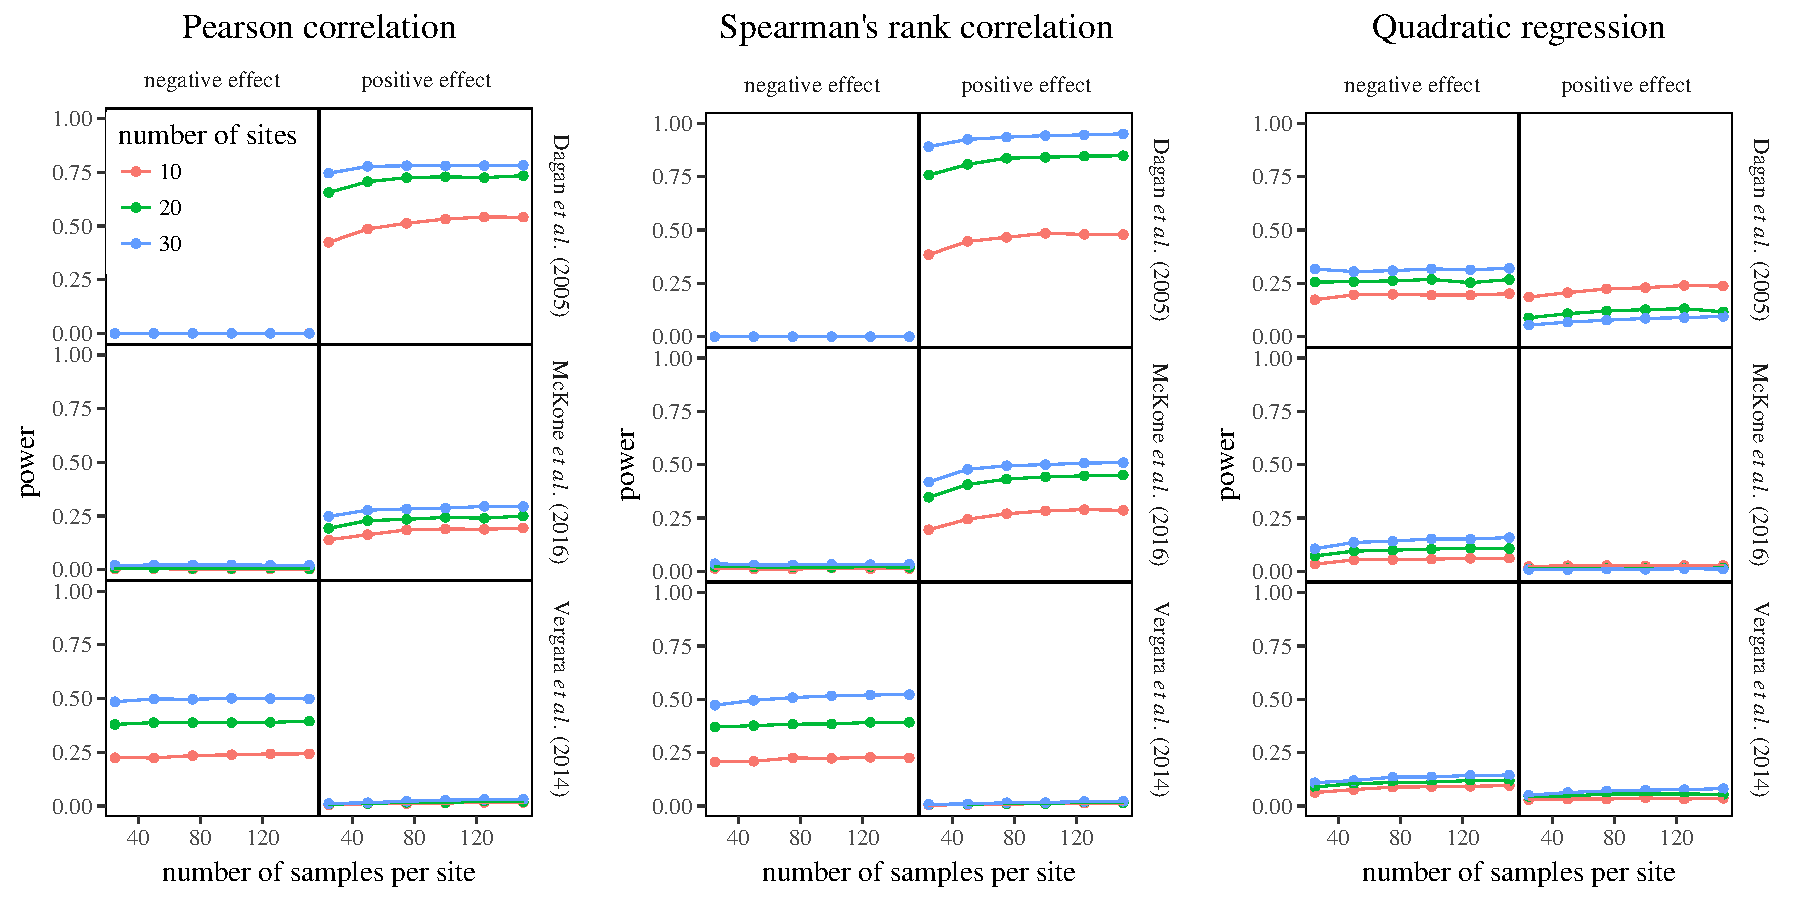
\includegraphics[width=1\textwidth]{../fig/power.pdf}
\caption{Power analysis for detecting a correlation and negative quadratic curvature.}
\end{figure}
\end{frame}

\begin{frame}{Discussion - Why low power?}
\begin{figure}
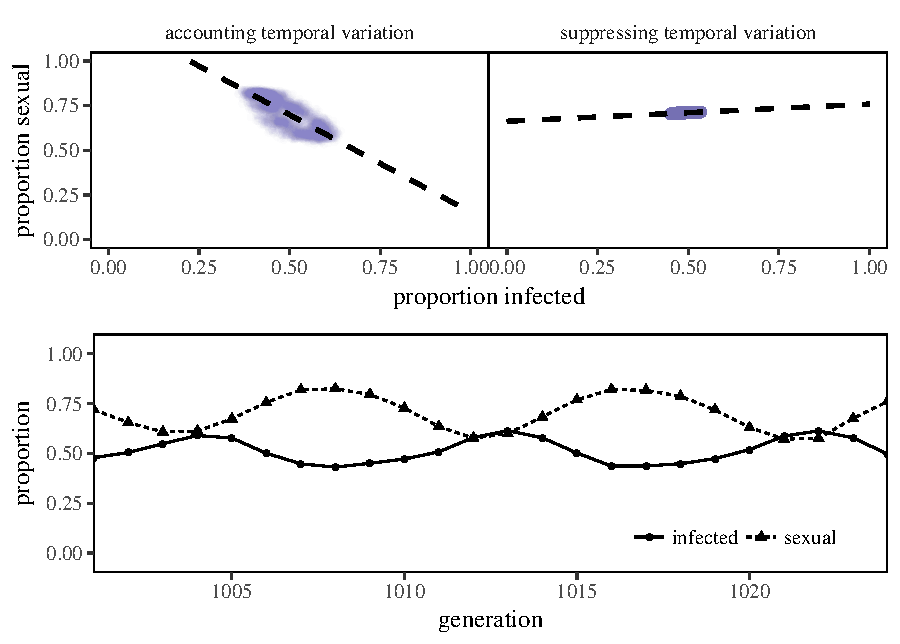
\includegraphics[width=0.8\textwidth]{../fig/cycle_example.pdf}
\caption{A sample data from a posterior sample. (left) type of cycles present in a simulated data (right) observed relationship v.s. expected relationship. (dashed line) quadratic regression.}
\vspace{-1em}
\end{figure}
\end{frame}

\begin{frame}{Discussion - Why low power?}
\begin{figure}
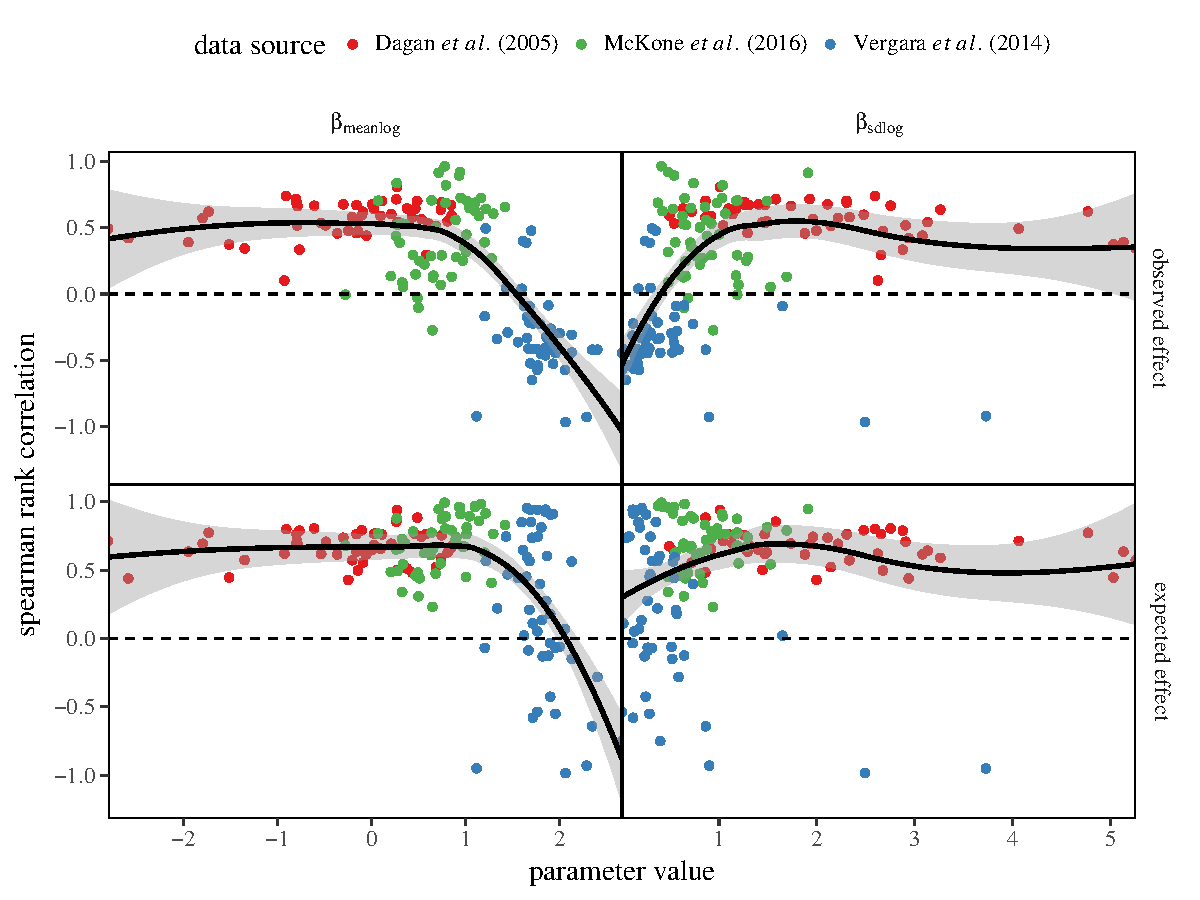
\includegraphics[width=0.8\textwidth]{../fig/sensitivity.pdf}
\vspace{-1em}
\caption{sensisivity plot of observed relationship v.s. expected relationship.}
\end{figure}
\end{frame}

\begin{frame}{Conclusion/questions}
\begin{itemize}
    \item Red Queen hypothesis not appropriate for Dagan \etal\ data? (high asexual diversity, highly interconnected but diverse habitats, strong drift by seasonal flood \cite{ben2007temporal})
    \item spatial data provides limited information; only Vergara \etal\ \cite{vergara2014infection} had spatiotemporal data
    \item identify different cycles in nature?
    \item is there a way to detect the Red Queen cycles from a spatiotemporal data? or account for cycles in a spatial data?
    \item consider pluralistic approach (Red Queen hypothesis + other mechanisms for maintaining sex)?
\end{itemize}
\end{frame}

\begin{frame}{Reference}
\tiny{
%% Add numbered references
\setbeamertemplate{bibliography item}[text]
%% Stop line breaks
\setbeamertemplate{bibliography entry title}{}
\setbeamertemplate{bibliography entry location}{}
\setbeamertemplate{bibliography entry note}{}
\bibliographystyle{unsrt}
\bibliography{../misc/redqueen}
}
\end{frame}
    
\end{document}
